\documentclass[14pt, aspectratio=169]{beamer}
\usetheme{Copenhagen}

\usepackage{graphicx}
\usepackage{forest}
\usepackage{tikz}
\usetikzlibrary{positioning}

\title{Knuth-Bendix Completion for\\ Program Optimization}
\subtitle{Thesis Proposal}
\author{Michael Schifferer}
\date{20.08.2025}


\begin{document}
	\maketitle
	
	\begin{frame}{What Kind of Optimization?}
		\begin{columns}
			\column<1->{0.5\textwidth} 

				Rewrite rules:\\
			R1: $0 + X \rightarrow X$\\
			R2: $X + 0 \rightarrow X$\\
			R3: $-X + X \rightarrow 0$\\
			R4: $(X +Y) + Z \rightarrow X + (Y + Z)$
			
				\column{0.5\textwidth} 
					\begin{minipage}[c][1\textheight][c]{\linewidth}
					\begin{forest}
					for tree={
						draw,                   % draw boxes around nodes
						rounded corners,        % rounded node corners
						align=center,           % center text
						edge={->},              % arrows for edges
						parent anchor=south,    % connect edges from bottom of parent
						child anchor=north,     % connect edges to top of child
						l sep+=15pt,            % increase level separation
						s sep+=10pt             % increase sibling separation
					}
					[$(--a + (-a)) + a$
					[$0 + a$, edge label={node[midway, right]{R3}}
					[$a$, edge label={node[midway, right]{R1}}, label=right:{\textcolor{green}{\checkmark}}]]
					]
				\end{forest}
			\end{minipage}
			\end{columns}
			\end{frame}
			\begin{frame}{What's the Problem?}
				\begin{columns}
					\column{0.5\textwidth}
					
						Rewrite rules:\\
					R1: $0 + X$ \only<1-2>{$\rightarrow$}\only<3->{\alert{$\leftrightarrow$}} $X$\\
					R2: $X + 0$ \only<1-2>{$\rightarrow$}\only<3->{\alert{$\leftrightarrow$}} $X$\\
					R3: $-X + X$ \only<1-2>{$\rightarrow$}\only<3->{\alert{$\leftrightarrow$}} $0$\\
					R4: $(X +Y) + Z$ \only<1-2>{$\rightarrow$}\only<3->{\alert{$\leftrightarrow$}} $X + (Y + Z)$
					
					\column{0.5\textwidth} 
					\begin{minipage}[c][1\textheight][c]{\linewidth}
						 \only<1>{\begin{forest}
					for tree={
						draw,                   % draw boxes around nodes
						rounded corners,        % rounded node corners
						align=center,           % center text
						edge={->},              % arrows for edges
						parent anchor=south,    % connect edges from bottom of parent
						child anchor=north,     % connect edges to top of child
						l sep+=15pt,            % increase level separation
						s sep+=10pt             % increase sibling separation
					}
					[$(--a + (-a)) + a$
					[$--a + ((-a) + a)$, edge label={node[midway,left]{R4}}
					[$--a + 0$, edge label={node[midway,left]{R3}}
					[$--a$, edge label={node[midway,left]{R2}}, label=right:{\textcolor{red}{\text{X}}}]
					]]
					[$0 + a$, edge label={node[midway, right]{R3}}
					[$a$, edge label={node[midway, right]{R1}}, label=right:{\textcolor{green}{\checkmark}}]]
					]
			\end{forest}}
		\only<3>{
			\centering\alert{Turns our nice DAG into an infinite undirected graph}
		}
		\vspace{1cm}
		\hspace{2cm}
			\only<2>{\begin{forest}
				for tree={
					draw, rounded corners, align=center,
					edge={->}, parent anchor=south, child anchor=north,
					l sep+=15pt, s sep+=10pt
				}
				[$--a$, label=south:{\text{?}}
				]
			\end{forest}}
		\end{minipage}
			\end{columns}

	\end{frame}
	
	\begin{frame}{Equality Saturation}
	\begin{columns}
		\column{0.3\textwidth}{
		\only<1>{$(--a + (-a)) + a$}
		\only<2>{\includegraphics[height=0.8\textheight,keepaspectratio]{/home/michi/Documents/thesis/KBC/prop_talk/files/e_graph1.png}}
		\only<3>{\includegraphics[height=0.8\textheight,keepaspectratio]{/home/michi/Documents/thesis/KBC/prop_talk/files/e_graph2.png}}
		\only<4>{\includegraphics[height=0.8\textheight,keepaspectratio]{/home/michi/Documents/thesis/KBC/prop_talk/files/e_graph3.png}}
		\only<5>{\includegraphics[height=0.8\textheight,keepaspectratio]{/home/michi/Documents/thesis/KBC/prop_talk/files/e_graph4.png}}}
		\column{0.4\textwidth}
		\centering
		\only<1-4>{\begin{tikzpicture}[node distance=1cm,>=latex]
			\coordinate (A) at (0,0);
			\coordinate (B) at (3,0);
			\draw[->,thick] (A) -- (B) node[midway,above]{\small \only<1>{to e-graph}\only<2>{$(X +Y) + Z \rightarrow X + (Y + Z)$}\only<3>{$-X + X \rightarrow 0$}\only<4>{$0 + X \rightarrow X$ and $X + 0 \rightarrow X$}};
		\end{tikzpicture}}
		\only<5>{contains}
		\column{0.3\textwidth}{
			\only<1>{\includegraphics[height=0.8\textheight,keepaspectratio]{/home/michi/Documents/thesis/KBC/prop_talk/files/e_graph1.png}}
			\only<2>{\includegraphics[height=0.8\textheight,keepaspectratio]{/home/michi/Documents/thesis/KBC/prop_talk/files/e_graph2.png}}
			\only<3>{\includegraphics[height=0.8\textheight,keepaspectratio]{/home/michi/Documents/thesis/KBC/prop_talk/files/e_graph3.png}}
			\only<4>{\includegraphics[height=0.8\textheight,keepaspectratio]{/home/michi/Documents/thesis/KBC/prop_talk/files/e_graph4.png}}}
			\only<5>{
				\begin{minipage}[c][.5\textheight][c]{1\linewidth}
					\hspace*{-2.5cm}
					{\begin{forest}
							for tree={
								draw,                   % draw boxes around nodes
								rounded corners,        % rounded node corners
								align=center,           % center text
								edge={->},              % arrows for edges
								parent anchor=south,    % connect edges from bottom of parent
								child anchor=north,     % connect edges to top of child
								l sep+=15pt,            % increase level separation
								s sep+=10pt,             % increase sibling separation
							}
							[$(--a + (-a)) + a$
							[$--a + ((-a) + a)$, edge label={node[midway,left]{R4}}
							[$--a + 0$, edge label={node[midway,left]{R3}}
							[$--a$, edge label={node[midway,left]{R2}}, label=right:{\textcolor{red}{\text{X}}}]
							]]
							[$0 + a$, edge label={node[midway, right]{R3}}
							[$a$, edge label={node[midway, right]{R1}}, label=right:{\textcolor{green}{\checkmark}}]]
							]
					\end{forest}}
			\end{minipage}}
	\end{columns}
	\end{frame}
\end{document}